\chapter{Photon production}
\label{photons}\index{Photon production}\index{photons}
\section{Photon conversion}
Photon conversion $q\rightarrow\gamma$ is similar to the conversion processes discussed in Section
 \ref{conversion}. A quark or anti-quark can convert into a high energy photon via
Compton or annihilation processes. All these processes are shown in Fig. \ref{fig:photonConv}.
\begin{figure}[htb]
  \begin{center}
    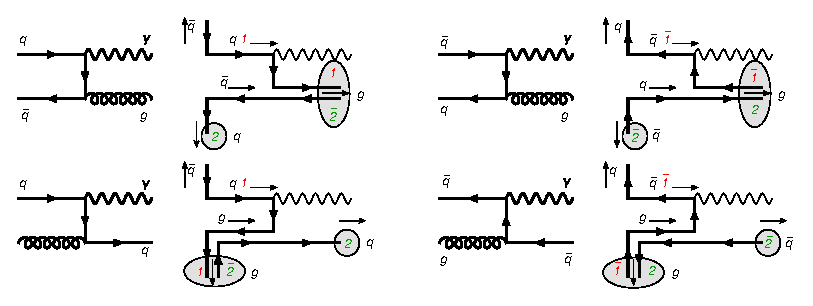
\includegraphics[width=16cm]{photonConversion1}
    \caption{$q\rightarrow \gamma$ and $\bar{q}\rightarrow \gamma$ 
      Feynman diagrams on the left and corresponding color lines on the right. 
      The upper part of each diagram represents the hard partons and photons, 
      the lower part the thermal partons.
      \label{fig:photonConv}}
  \end{center}
\end{figure}
The partons in the gray blobs are sampled from Fermi or Bose distributions, 
depending on their kind.

\section{Photon radiation}
\label{photonradiation}
The other included process is a quark emitting a photon $q\rightarrow q\gamma$ 
analogous to the previously described process of gluon emission 
(see Section \ref{radiative}).
Here, we do not have a complicated color structure to take care of. The quark 
of course keeps its color when emitting a photon. 
Please note that the transition rates do not include a factor of $(e_f/e)^2$, which 
is $4/9$ for up and $1/9$ for down and strange quarks. These factors are included 
in the main routine, when we actually know what kind of quark we have.
Everything else, such as the sampling of the rate using the rejection method, works
just like in the case of gluon emission.

The actual implementation is rather short because of he lack of need for color
indeces. Here is what is done when photon emission occurs:\\

\begin{boxedverbatim}
  else if( radiatePhoton == 1 ) // see if photon emission happens
  {
      // do process 4, q->qgamma
      f = rates->findValuesRejection(pRest/T, T, alpha_s, Nf, random, import, 4); 

      newOne.p(f.y*T*vecp.px()/vecp.pAbs()*boostBack,  // emitted gamma's momentum
      f.y*T*vecp.py()/vecp.pAbs()*boostBack,    // since the direction does not change 
      f.y*T*vecp.pz()/vecp.pAbs()*boostBack);   // I can use vecp here already

      newOne.id(22);                            // emitted parton is a photon
      newOne.mass(0.);
      newOne.frozen(1);
      newOne.x(x);                              // set the new parton's initial position
      newOne.y(y);
      newOne.z(z);
      plist[0]->push_back(newOne);              // add the photon to the list of partons 
  }
\end{boxedverbatim}\\

~\\
In 
#ReturnValue Rates::findValuesRejection(double u, double T, double alpha_s, int Nf,#\\
#                                         Random *random, Import *import, int process)#\\
process number 4 takes care of photon emission. See Section \ref{sampling} for details.


  
  

%%% Local Variables: 
%%% mode: latex
%%% TeX-master: "manual"
%%% End: 
